\chapter{Fundamentação Teórica}
\label{cap:fundamentacao-teorica}

\section{Processos e Threads}
\label{sec:processos-e-threads}

\subsection{Descritores de Arquivo}
% Falar de PCID

\subsection{Troca de Contexto}

\section{Espaço de Endereçamento Virtual}

\subsection{Modelo de Paginação}

\subsection{Modelo de Segmentação}

\subsection{Page Walk}

\subsection{TLB}
% Falar de TLB tagged

\subsection{Outros Mecanismos de Memória}
\label{sec:outros_mecanismos_memoria}
% TODO: Falar do Protected memory domain do arm

\section{Chamadas de Sistema}

\subsection{Modos de Programação e API}

\section{Device Drivers}
\label{sec:dd}

\section{Virtualização}
\label{sec:virtualizacao}

%TODO: Eu acho que faltou introduzir alguns dos termos básicos logo no início
% contar um pouco como funciona e acertar a fluídez do texto

A ideia de oferecer a abstrações de máquinas virtuais dentro de uma mesma
máquina é um aspiração de longa data como o emblemático trabalho de Popek e
Goldberg \cite{popek} demonstra. Este foi públicado em 1974 indicando os
requisitos necessários para a terceira geração processadores fornecessem
virtualização completa. Neste período se tinha noção de algumas das vantagens
que a virtualização por software e hardware poderia entregar. Dentre as
inúmeras vantagens da virtualização destacam-se a possibilidade de executar
aplicações legadas em um SO antigo, recursos que facilitam o processo de
desenvolvimento de software, serviços de núvem, \emph{checkpoints}, migração de
processos, isolamento, dentre outras.

O elemento central da virtualiação é o \emph{Virtual Machine Monitor (VMM)}
(também conhecido como \textbf{hypervisor}) que é responsável por criar a
ilusão de múltiplas máquinas em um mesmo hardware físico \cite{tanenbaum}.
Essas máquinas virtuais rodando sobre o mesmo hardware tem a capacidade de
executar diferentes SOs. Complementarmente a estes conceitos, existe a ideia de
máquina convidada (\emph{guest}) e máquina hóspede (\emph{host}). O primeiro
refere-se ao SO que está executando sobre o VMM e o segundo refere-se a máquina
que está executando sobre o hardware com privilégios.

Um dos objetivos da virtualização consiste em permitir que um SO inicialize
como se estivesse dando boot em uma máquina real. Para que isso seja possível é
preciso emular o hardware de forma que o \emph{guest} não perceba que está em
um mecânismo simulado; ao mesmo tempo este processo deve ocorrer de forma
eficiênte. Em 1974, \citep{popek} sugeriram alguns requisitos para que os
hardware modernos dessem suporte completo para virtualização, esses conceitos
são amplamente implementados nos processadores modernos. Basicamente os autores
destacam que três dimênsões que devem ser consideradas para fornecer a
virtualização completa no nível dos processadores: segurança, fidelidade e
eficiência.

No que tange o assunto segurança, o VMM deve ter total controle sobre os
recursos virtualizados. Uma opção é utilizar um interpretador que intercepta
cada instrução e realiza exatamente o que a instrução precisa. Algumas
instruções podem ser executadas diretamente, mas outras não, por exemplo, não
deve ser possível para a máquina \emph{guest} desativar as interrupções de toda
a máquina \cite{tanenbaum}. Para contornar tal situação, o o SO \emph{guest}
deve ter a ilusão de que as interrupções estão desativadas.

Do ponto de vista da fidelidade, o comportamento do programa executando na
máquina virtual deve comportar-se de forma idêntica a se estivesse executando
diretamente no hardware. Na prática existem várias complicações associadas a
este requisito que levam a categorização das instruções utilizadas pela CPU em
três grupos de diferentes:

\begin{itemize}
  \item \textbf{Instruções sensíveis}: CPUs que fornecem \emph{user mode} e
        \emph{kernel mode} apresentam instruções comuns para ambos os modos de
        operação, mas que tem comportamentos diferentes dependendo de cada modo
        de operação no qual a instrução é executada;
  \item \textbf{Instruções privilégiadas}: São instruções que geram uma
        \emph{trap} quando executado no modo usuário, mas que não geram
        \emph{trap} em modo Kernel;
  \item \textbf{Instruções de controle de fluxo sensíveis}: São aquelas que
        tentam mudar a configuração de algum recurso do sistema.
\end{itemize}

Se você tentar fazer algo em modo usuário que você não deveria ser capaz de
fazer, o hardware deve capturar essa ação; em outras palavras, Popek e Goldberg
mostraram que uma máquina é virtualizável se o conjunto de instruções sensíveis
é um subconjunto das instruções privilégiadas. Apesar de parecer um conceito
simples, levaram-se vários anos para que as CPUs incorporassem tais definições
e assim oferecessem um adequado suporte de hardware para a virtualização.

O suporte completo para a virtualização em hardware foi resolvido apenas em
2005 pela intel \cite{uhlig} com uma técnologia chamada \textbf{Virtualization
Technology (VT-x)}. A AMD tem uma solução parecida chamada \textbf{Secure
Virtual Machine (SVM)}. A ideia básica é criar um invólucro no qual a máquina
virtual pode executar um SO \emph{guest} iniciado dentro deste recipiente, o SO
contínua lá até que provoque uma \emph{trap} que faz com que o VMM tenha que
lidar com a situação. O conjunto de instruções que provocam uma \emph{trap} são
controlados por um conjunto de bits na qual o VMM tem acesso, essa extensão
torna possível a execução classíca de uma máquina virtual baseada em
"interrupção-e-emulação" \cite{tanenbaum}.

Do ponto de vista da eficiência, a virtualização deve fazer com que a maior
parte do código executado pelo SO \emph{guest} não sofra interferêcia do VMM.
Uma das abordagens utilizada antes de se ter o hardware de virtualização foi a
adoção de técnicas na qual o hypervisor interceptava as instruções e as
reescrevia em tempo de execução com uma sequência de código considerada segura.
Esse mecânismo permitia substituir instruções sensíveis, mas não privilégiadas;
tal técnica ficou conhecida como \textbf{tradução binária} e demostrou-se
extremamente eficiênte devido ao seu sofisticado mecânismo de \emph{cache}.

% TODO: Falar dos tipos de hypervisor
%FIGURA X

\subsection{A tecnologia VT-x}

Em 2005 Uhlig \citep{uhlig} apresentaram a tecnologia de virtualização adotada
pela Intel para fornecer a virtualização completa no nível do processador. Na
Figura \ref{fig:vt-x_flow} podemos notar os elementos presentes em tal
tecnologia e como eles interagem, dois novos modos de operações foram
introduzidos nas CPUs: \emph{VMX non-root} e \emph{VMX root}.

\begin{figure}[!h]
  \centering
  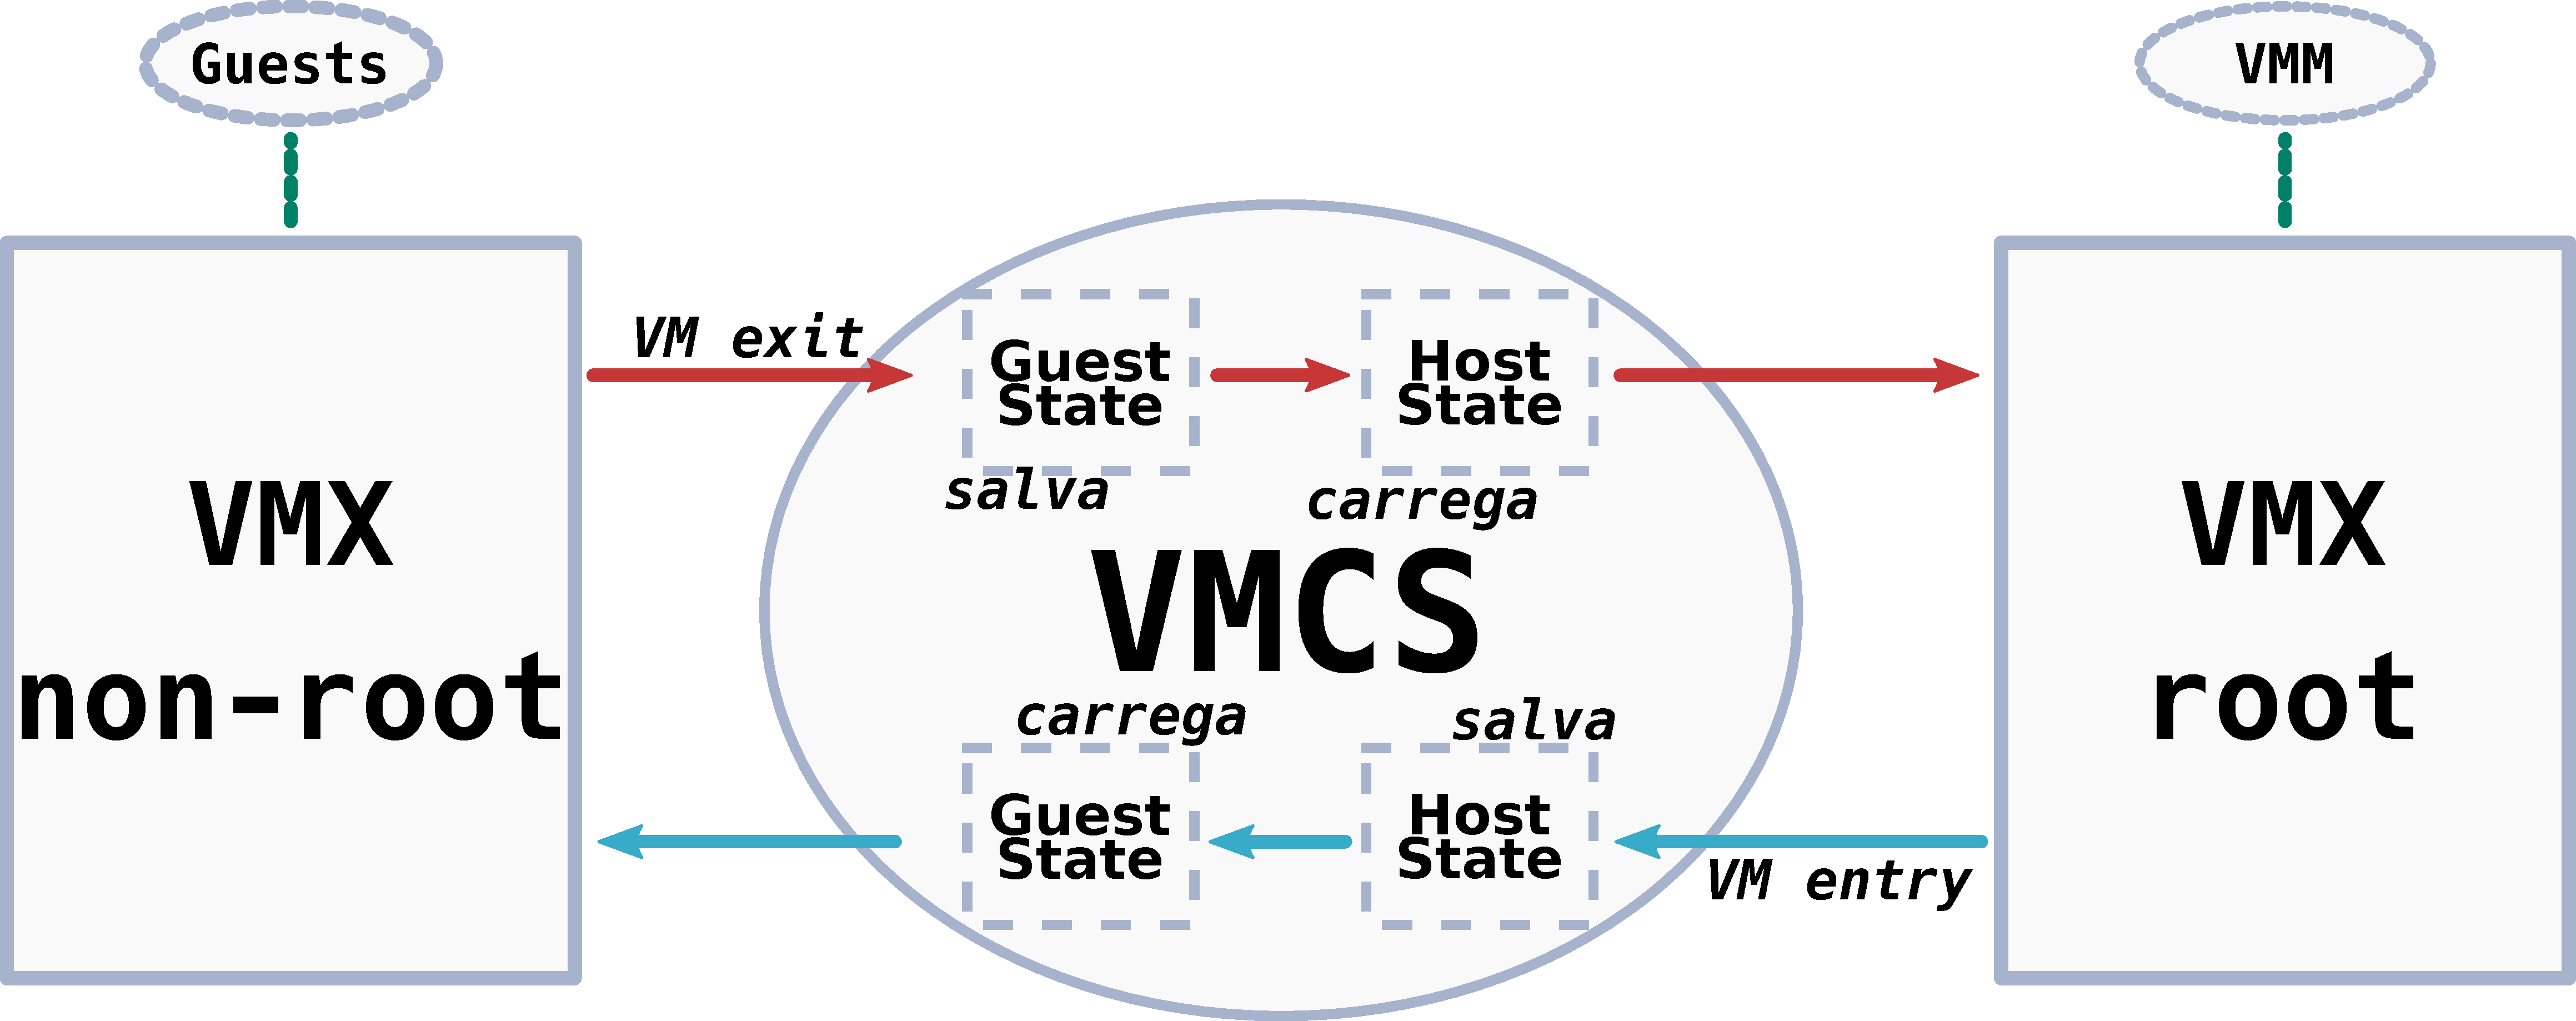
\includegraphics[width=0.6\textwidth]{vt-x_flow} 
  \caption{Fluxo do comportamento da tecnologia VT-x}
  \label{fig:vt-x_flow}
\end{figure}

O \emph{VMX non-root} é o modo de operação na qual a máquina \emph{guest}
executa, enquanto o \emph{VMX root} é o modo de operação utilizado pelo VMM. É
interessante observar que os dois modos tem suporte para os quatro níveis de
privilégios fornecidos pelos processadores Intel, isto permite que a máquina
\emph{guest} que tente executar uma instrução privilégiada em algum desses
nível forneçam tal informação para o VMM. Contudo, os software executando como
\emph{VMX non-root} são desprivilégiados de certa forma, a não pelo nível de
privilégios. Note da Figura \ref{fig:vt-x_flow} que existe uma trasição chamada
\emph{VM exit} e \emph{VM entry}. A transição \emph{VM exit} ocorre quando o
controle é transferido do \emph{guest} para o VMM, isto faz com que o estado da
máquina \emph{guest} seja salvo e o estado do \emph{host} seja carregado para
que o VMM decida como tratar a interrupção. No sentido oposto, ocorre a
transição \emph{VM entry} na qual o VMM transfere o controle para a máquina
\emph{guest}, para isto ela salva o estado do \emph{host} e carrega o estado
anterior do \emph{guest}. Todas as informações referentes a virtualização são
mantidas em uma estrutura de dados chamadas de \emph{virtual-machine control
structure (VMCS)} que basicamente tem por função gerenciar as transições entre
a \emph{VM entry} e \emph{VM exit}.


